\documentclass{article}
\usepackage[utf8]{inputenc}
\usepackage{amsmath}
\usepackage{amsthm}
\usepackage{amsfonts}
\usepackage{parskip}
\setlength{\parindent}{0em}
\setlength{\parskip}{1em}
\usepackage{algorithm}
\usepackage{algpseudocode}
\usepackage{graphicx}
\usepackage{systeme}
\usepackage{tikz}
\usepackage[
backend=biber,
style=ieee,
sorting=ynt
]{biblatex}
\usepackage{pdfpages}

\addbibresource{specification.bib}

\title{Optimisation of parallel KD-trees using heuristics for neural networks simulation \\ Project Specification - Degree Project in Computer Science, DD150X}
\author{Daniel Benedí \\ Supervisor: Alexander Kozlov}
\date{February 2022}


\begin{document}
\maketitle

\section*{Introduction}
In the last decade neurology has been benefited of simulating the nerve cell
behaviour or neural networks. This made use of large-scale, high-precision 
experimental methods of data acquisition which allowed to develop realistic tools
to understand the brain functions and diseases \cite{MARKRAM201139}. Due to the
amount of data collected, this simulations have to be handled with supercomputers
to integrate different levels of simulation. Even though they are using high-performance
computers, it is not possible to fully simulate a human brain \cite{FURBER2006},
and because of that it is used only sub-regions of the hole structure. This study
will try to optimise the performance obtained by this simulations focusing on how
to improve the acquisition of sub-regions using some techniques from computer
graphics.

\section*{Problem Statement}
In computer graphics, there are several approaches for constructing kd-trees for
ray-tracing. The reasons they are used are also applied for this problem so they
require a spatial localisation around a big cloud of points. Some of this are
parallel KD-trees that are optimised with some heuristic to get a better performance
\cite{CHOI2010}. Using this, we pose the question: "Which parameterised heuristics
can work better with parallel kd-trees for neurological simulation?".

\section*{Approach}
To check how effective are this heuristics, we are going to have several approaches
to the problem. First of all, it will be implemented with the traditional
algorith \cite{Adamsson_Vorkapic_2016}, massively parallel KD-tree construction
\cite{7169256} and some other approaches of constructing this massively parallel
KD-trees aided with some heuristics such as Surface Area Heuristic \cite{CHOI2010}
or Curve Complexity Heuristic \cite{LU2021}, this heuristics may need some little
changes to be more related to the actual problem.

The evaluation of this methods will be based on a dataset that will be based
on some existing real cases \cite{NeuroMorpho} and some little cases that
will be created by hand using the python library treem \cite{treem}. From this
dataset we will analyze different metrics such as execution time and cache misses

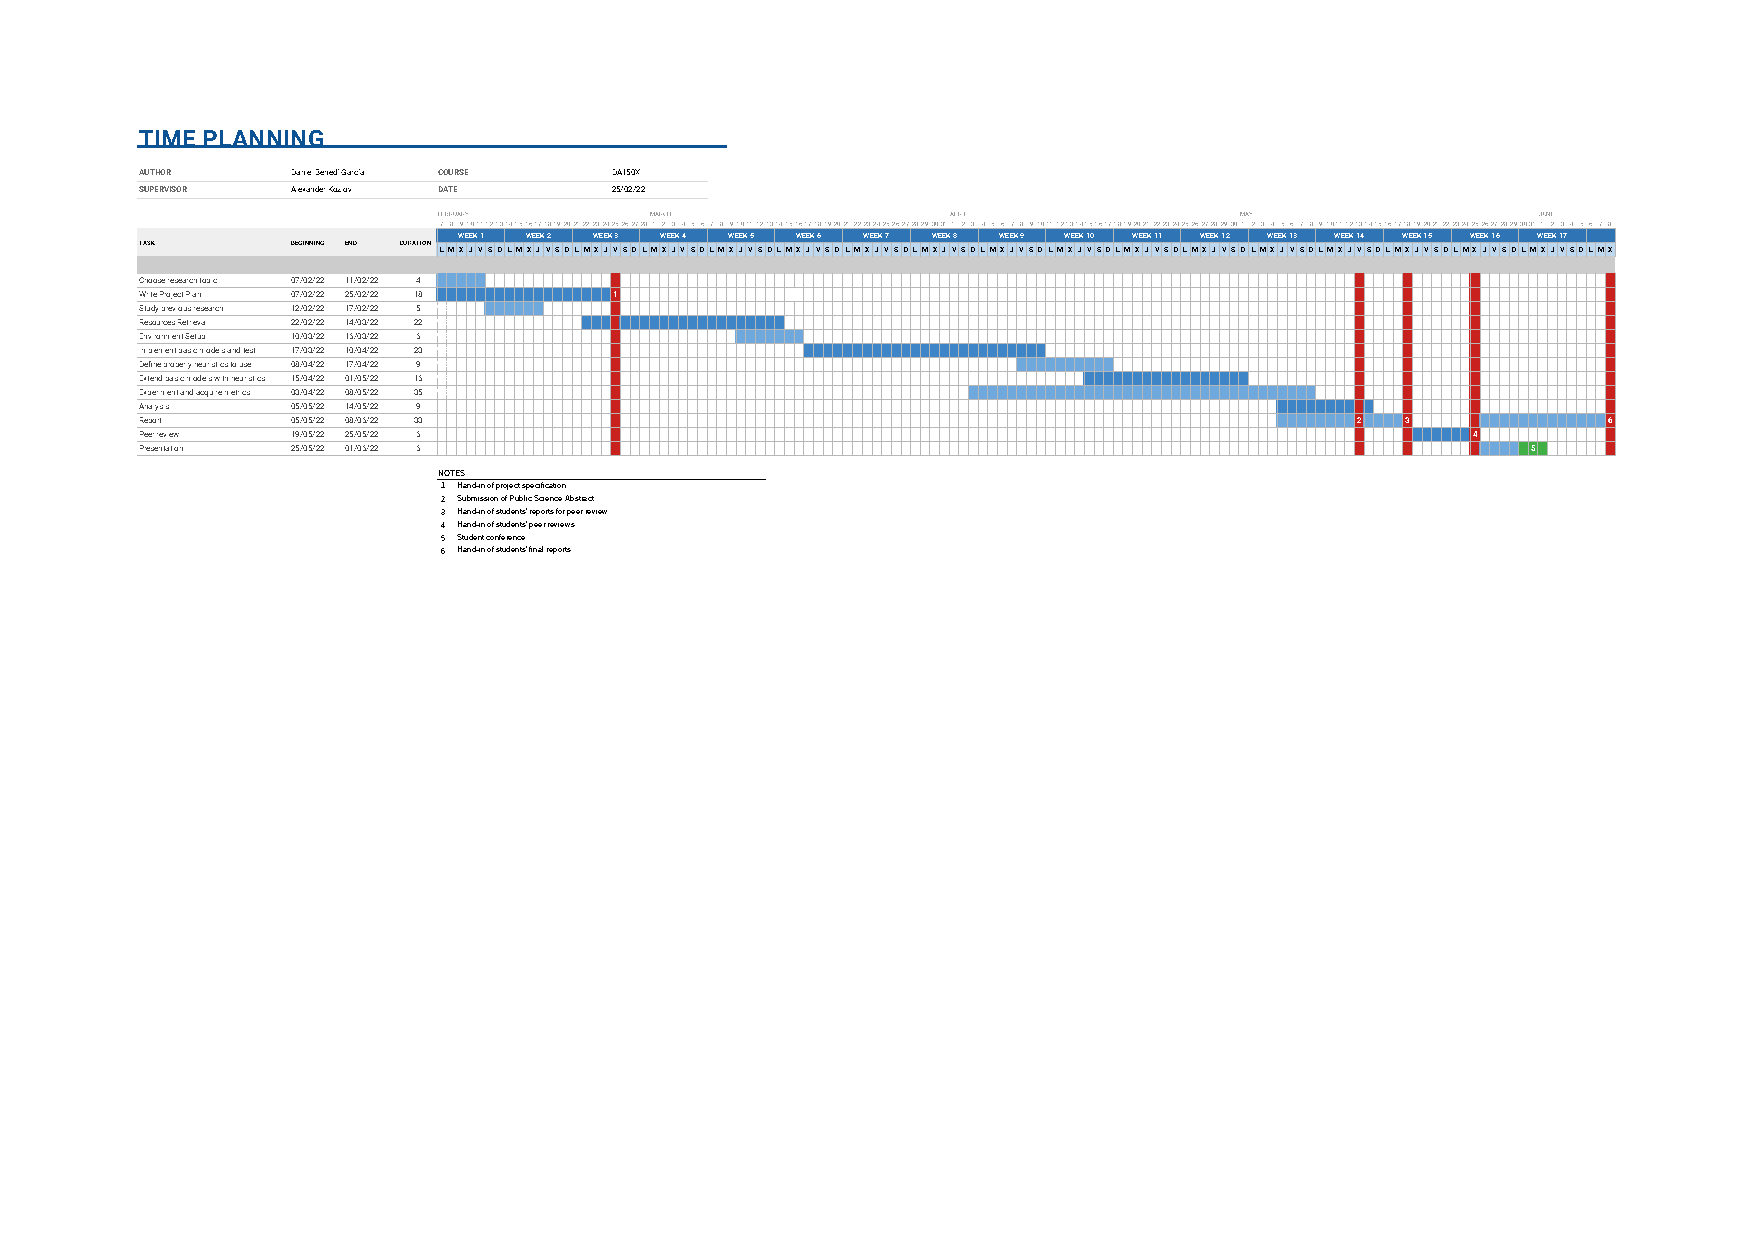
\includepdf[landscape=true,lastpage=1]{GanttDiagram.pdf}

\printbibliography

\end{document}

